% A skeleton file for producing Computer Engineering reports
% https://kgcoe-git.rit.edu/jgm6496/KGCOEReport_template

\documentclass[CMPE]{../KGCOEReport}

% The following should be changed to represent your personal information
\newcommand{\classCode}{CMPE 460}  % 4 char code with number
\newcommand{\name}{Andrei Tumbar}
\newcommand{\LabSectionNum}{2}
\newcommand{\LabInstructor}{Beato}
\newcommand{\TAs}{Xavier Brooks\\
Diana Yakobchuk\\
Charles Poliwoda}
\newcommand{\LectureSectionNum}{1}
\newcommand{\LectureInstructor}{Beato}
\newcommand{\exerciseNumber}{5}
\newcommand{\exerciseDescription}{MSP432 Timers, Interrupts, and Analog-to-Digital Converter}
\newcommand{\dateDone}{February 12th}
\newcommand{\dateSubmitted}{February 26th}

\usepackage{tikz}
\usepackage{circuitikz}
\usetikzlibrary{calc}
\usetikzlibrary{circuits.logic.IEC,calc}
\usepackage{multirow}
\usepackage{float}
\usepackage{lmodern}
\usepackage{siunitx}
\usepackage{subcaption}
\usepackage{graphicx}
\usepackage[usestackEOL]{stackengine}
\usepackage{scalerel}
\usepackage[T1]{fontenc}
\usepackage{amsmath}
\usepackage{pdfpages}

\ctikzset{logic ports=ieee}

\def\lbar#1{\ThisStyle{%
    \setbox0=\hbox{$\SavedStyle#1$}%
    \stackengine{2.2\LMpt}{$\SavedStyle#1$}{\rule{\wd0}{0.1\LMpt}}{O}{c}{F}{F}{S}%
}}

\DeclareFontFamily{U}{mathx}{\hyphenchar\font45}
\DeclareFontShape{U}{mathx}{m}{n}{ <-> mathx10 }{}
\DeclareSymbolFont{mathx}{U}{mathx}{m}{n}
\DeclareFontSubstitution{U}{mathx}{m}{n}
\DeclareMathAccent{\widebar}{\mathalpha}{mathx}{"73}

\makeatletter
\newcommand{\cwidebar}[2][0]{{\mathpalette\@cwidebar{{#1}{#2}}}}
\newcommand{\@cwidebar}[2]{\@cwideb@r{#1}#2}
\newcommand{\@cwideb@r}[3]{%
    \sbox\z@{$\m@th\mkern-#2mu#3\mkern#2mu$}%
    \widebar{\box\z@}%
}
\newcommand\currentcoordinate{\the\tikz@lastxsaved,\the\tikz@lastysaved}
\makeatother

\newcommand\decbin[9]{%
    \par\smallskip
    \makebox[3cm][r]{$#1$\ }\fbox{#2}\,\fbox{#3}\,\fbox{#4}\,\fbox{#5}\,\fbox{#6}\,\fbox{#7}\,\fbox{#8}\,\fbox{#9}\par}


\def\code#1{\texttt{#1}}

\ctikzset{resistors/scale=0.8}

\ctikzset{logic ports/scale=0.7}

\begin{document}
    \maketitle
    \section*{Abstract}

    In this laboratory exercise, multiple hardware peripherals were configured for
    operation on the MSP432 board. The hardware buttons or switches were used in
    interrupt mode to use less CPU time polling the hardware.
    The set of two Timer32 were configured with arbitrary interrupt callbacks as
    well as the systick timer built into the ARM chip. The analog-to-digital (ADC)
    converter was configured to operate on an external pin to measure voltages from
    sensors and other devices. A combination between the timers and the ADC was used
    to operate a line-scan camera using the proper timing on the control pins and ADC pin.

    \section*{Design Methodology}

	\subsection*{Interrupts}

	Hardware interrupts are CPU level signals that will interrupt the normal execution
	of the processor. The current running context of the processor will be saved to
	the stack and the context is switched to the interrupt handler. Interrupt in this
	lab exercise were used to handle the button presses on the physical board. To keep
	things simple for the user, a function pointer is passed in during switch
	initialization to register a callback for interrupt handling. The switch can also
	be configured to interrupt on button press, release or both. 

	\subsection*{Timers}

	The MSP432 board is equipped with three sets of general purpose timer peripherals.
	The SysTick timer is a peripheral shipped with every ARM chip and is most commonly
	used for preemption in real-time operating systems as well as keeping time for
	many embedded systems. The other two timers, Timer32 and TimerA are peripheral on
	the board instead of the ARM chip. This exercise will focus on the operation of the
	Timer32 timers. These timers are 32 or 16-bit downcounting timers that can generate
	interrupts when reaching zero.\\

	A driver was written for the Timer32 peripheral in which the reload value and the
	prescaler can be set to interrupt at different periods. The prescaler or clock
	divider on the Timer32 has three supported values 1, 16 and 256.
	Using a chosen prescaler an the system clock speed, a timer reload value can be
	calculated to cause the timer to interrupt at the desired frequency. In addition to
	a reload value being calculated, during timer initialization an interrupt callback
	is also registered with the timer (both for SysTick and Timer32) where a configurable
	interrupt handler may be used. This allows a clean initialization process of the
	hardware timers to operate with interrupts.

    \subsection*{ADC}

	The analog-to-digital converter is a peripheral device that will digitize an analog
	voltage using a reference voltage. The device uses a digital-to-analog converter
	and a op-amp in a comparator configuration to resolve the voltage. The ADC will
	require a conversion time after it is signaled to begin measuring the external pin
	voltage. When this time is complete, a flag will be set (and optionally a
	interrupt fired) telling the programmer that the register holding the ADC digital
	value is ready to be read.\\

	The initialization of the ADC is straightforward and doesn't require any parameters.
	The registers on the peripheral are simply set to use the \SI{2.5}{\volt} internal 
	reference voltage as well use the 14-bit conversion mode. These settings meant that
	values from the ADC would range from $0$ to $2^{14} - 1$ or $16383$. The minimum value
	would mean the ADC read \SI{0}{\volt} on the external pin while the maximum would
	signify the reference voltage in this case \SI{2.5}{\volt}.

	\subsection*{Line-scan Camera}

	The final portion of this exercise involved operating the line-scan camera with the
	timers and ADC peripherals. The camera operate with three pins:
	\code{SI}, \code{CLK} and \code{ADC} pins. The \code{SI} and \code{CLK} pins
	are input pins controlled by the MSP432 board. The \code{CLK} pin is a clock
	signal (square wave) with a rising edge trigger that will provide a synchronization
	on the \code{ADC} output pin when reading values from the line-scan sensor.
	The timing of the control pins on this camera had a very strict set of rules to
	operate properly. A state machine was designed to process each image read from
	the camera.

	\begin{figure}[h!]
        \centering
        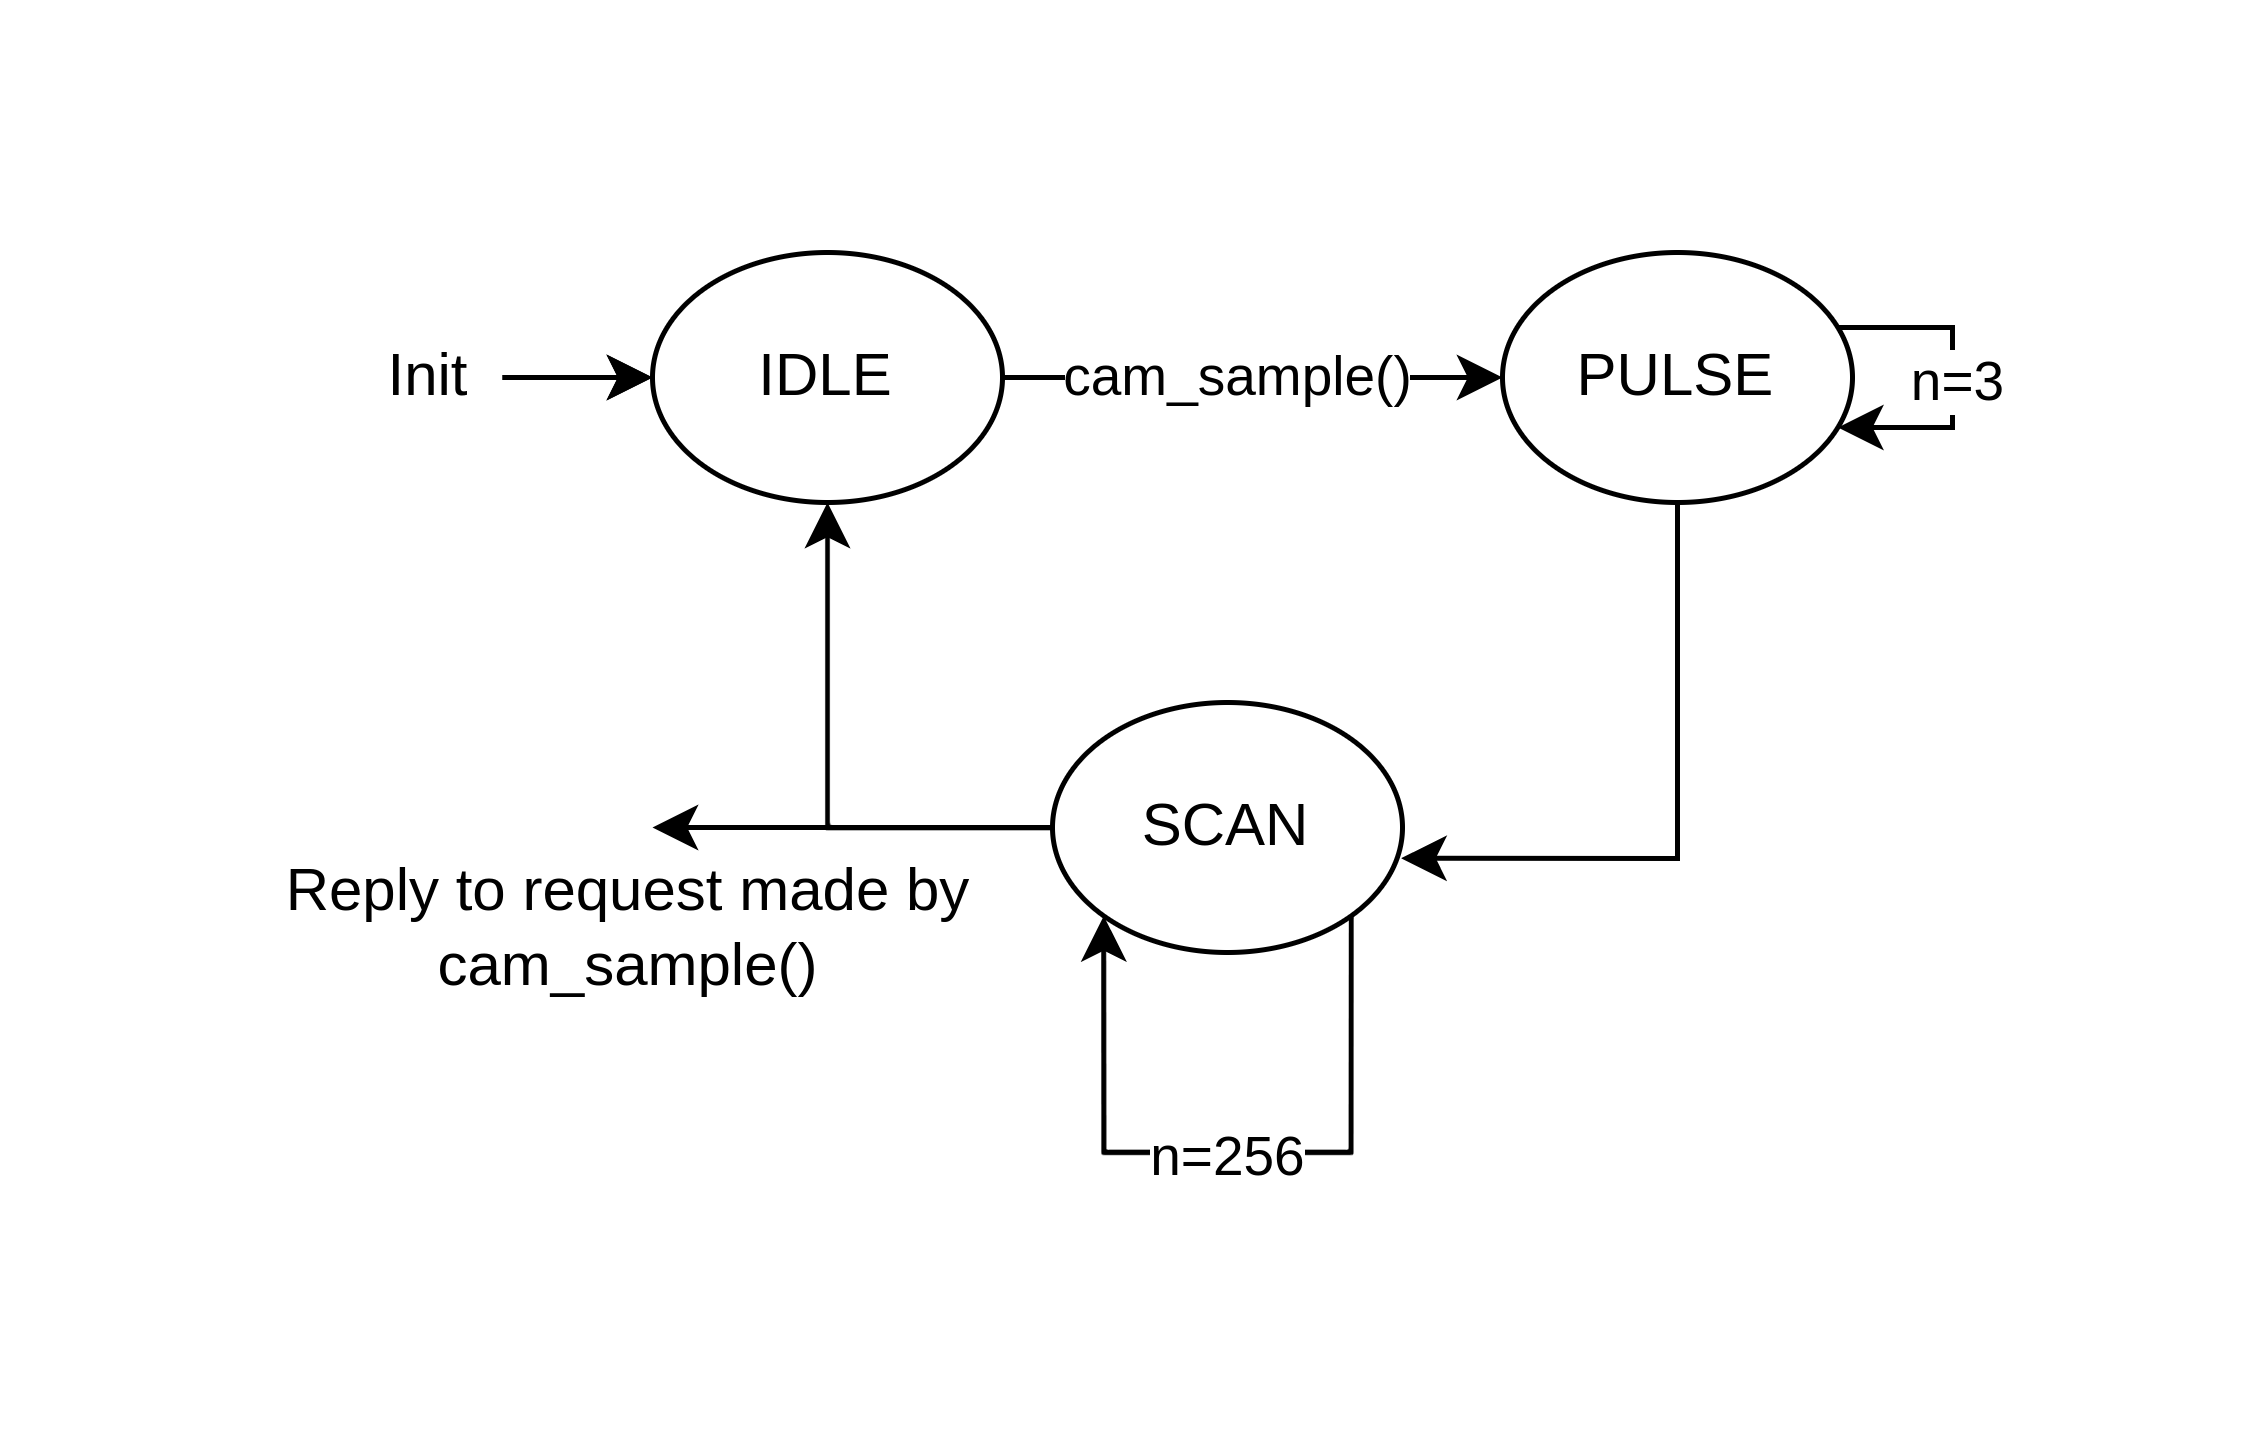
\includegraphics[width=12cm]{cam_state}
        \caption{Camera state machine used to provide timing on control signals.}
        \label{fig:cam_state}
	\end{figure}

	Each state shown in the diagram was run by a "tick" function called from the
	SysTick interrupt handler. Because the camera clock signal was chosen to be run
	at \SI{100}{\kilo\Hz}, The SysTick timer was configured to run at double this
	frequency so that the clock signal could be set both high and low. An internal
	counter in addition to the current state of the state machine kept track of
	the current tick index in the running state. During the \code{PULSE} state,
	the \code{SI} pulse and initial \code{CLK} signal are sent to the camera. By
	setting a rising edge on the clock while the \code{SI} signal is high the camera
	begins to integrate. The next \code{SI} pulse will then signal the camera to place
	the line-scan pixel readings in a buffer and will be clocked out during the next
	128 clock cycles to the ADC output pin. One of the Timer32 timers is used to provide
	the timing between the \code{SI} pulses while the SysTick (as previously mentioned)
	will provide each tick during the camera running states.

	\subsection*{Issues}

	When writing the SysTick timer driver, I ran into an interesting problem where the
	\code{SysTick\_Handler} function could not be overridden inside the \code{tim}
	driver. \code{tim} is where the timers are initialized and controlled.
	To give more context, all drivers I write for the MSP432 board are compiled
	separately as a static libraries and linked into a binary as needed.
	The issue arises from the fact
	that all the interrupt handlers are declared with \code{\_\_attribute\_\_((weak, alias("Default\_Handler")))} which will tell the linker to call \code{Default\_Handler}
	if the interrupt IRQ is not overridden. By the time you are at the link step of the
	compilation pipeline, the weak reference is dropped for symbol it is point to. It is
	therefore up to the linker to choose between the symbol from the binary or that
	from the static library. For some reason,
	the linker decided not to override the \code{SysTick\_Handler} interrupt while the
	Timer32 handlers were overridden. To fix this issue, \code{SysTick\_Handler} was
	defined the project's \code{main.c} and a \code{cam\_irq} function was exposed to
	be called by the SysTick interrupt. \\

	When testing the camera signal output, the oscilloscope could not properly autoscale
	to the camera output pin. This was because the oscilloscope autoscale will attempt
	to find a period signal and then scale the viewer to this signal. The issue with
	the camera output is that even though these is an underlying periodic signal
	seen by each exposure cycle, there is also a large amount of higher frequency
 	signals that cause the oscilloscope to zoom far past what is required. To fix this
 	issue, the \code{SI} signal was connected to the second probe to allow the scope to
 	autoscale to this signal instead.

    \section*{Results}


	\section*{Analysis}

	The time measured by the timer peripheral can be modeled by Equation \ref{eq:gen}.
	
	\begin{equation}
	t = \frac{prescaler}{f_{clk}} \cdot n_{count}
	\label{eq:gen}
	\end{equation}

	The shortest amount of measurable time is based on the CPU clock speed. If a single
	count on the timer peripheral is measured with no prescaler at \SI{48}{\mega\hertz}
	clock rate, \SI{20}{\nano\s} (Equation \ref{eq:short}).
	This of course is also limited by the instruction overhead required to measure a
	single clock cycle.

	\begin{equation}
	t_{short} = \frac{1}{\SI{48}{\mega\hertz}} \cdot 1 = \SI{20}{\nano\s}.
	\label{eq:short}
	\end{equation}

	The longest time measurable using
	a timing peripheral is with the maximum prescaler of 256 and the slowest clock speed
	of \SI{1.5}{\mega\hertz}, the 32-bit counter will overflow at $2^{32} - 1$.

	\begin{equation}
	t_{long} = \frac{256}{\SI{1.5}{\mega\hertz}} \cdot (2^{32} - 1) = \SI{8.48}{days}.
	\label{eq:long}
	\end{equation}

	The maximum time can also be extended by ``daisy'' chaining multiple 32-bit integers
	together to keep track of longer time intervals.

    \section*{Conclusion}

	

	\section*{Questions}

	\begin{enumerate}
	\item
	IRQ flags need to be cleared in the interrupt service routine because otherwise
	the CPU could immediately interrupt again and essentially be forever block inside
	the interrupt.
	\item
	Different interrupts will run different ISRs. For example, there is a unique ISR for
	each switch on the board. If the peripheral uses the same ISR for multiple pins,
	a unique flag will be set in one of the status or IRQ registers on the peripheral.  
	\item
	The initiation of the the camera data transfer happens in four distinct steps:
	\begin{enumerate}
	\item \code{SI} goes high,
	      \code{CLK} stays low
	\item \code{SI} stays high,
		  \code{CLK} goes high
	\item \code{SI} goes low,
		  \code{CLK} stays high
	\item \code{SI} stays low,
		  \code{CLK} goes low
	\end{enumerate}
	
	Each stage happens inside a distinct SysTick tick occuring at \SI{200}{\kilo\hertz}
	intervals.

	\end{enumerate}

\end{document}